\begin{figure}
\centering
\begin{subfigure}[t]{0.25\textwidth}
\centering
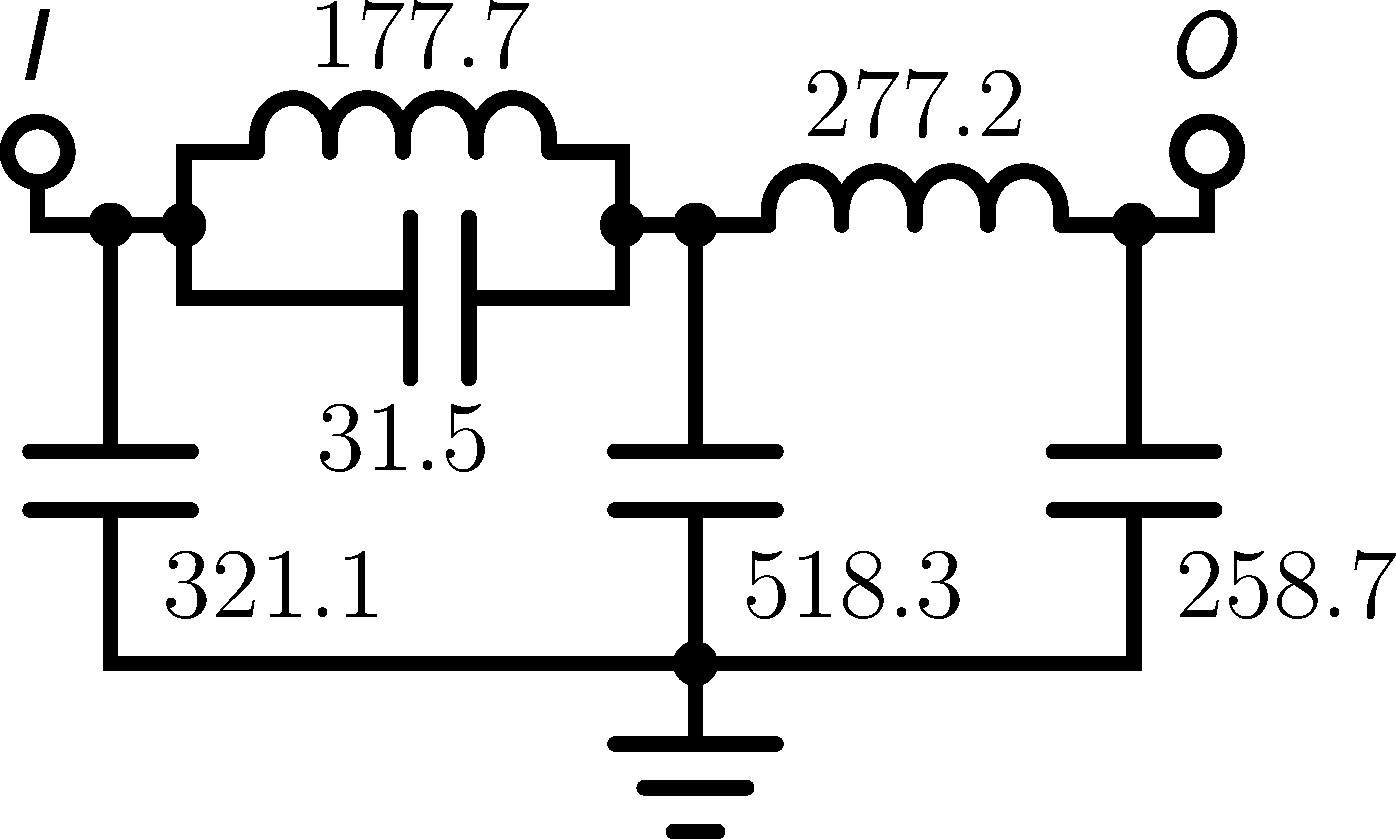
\includegraphics[scale = 0.14]{../ch6/figures/lpf3_circuit1}
\caption{\label{fig:lpf3_circuita}}
\end{subfigure}%
\begin{subfigure}[t]{0.25\textwidth}
\centering
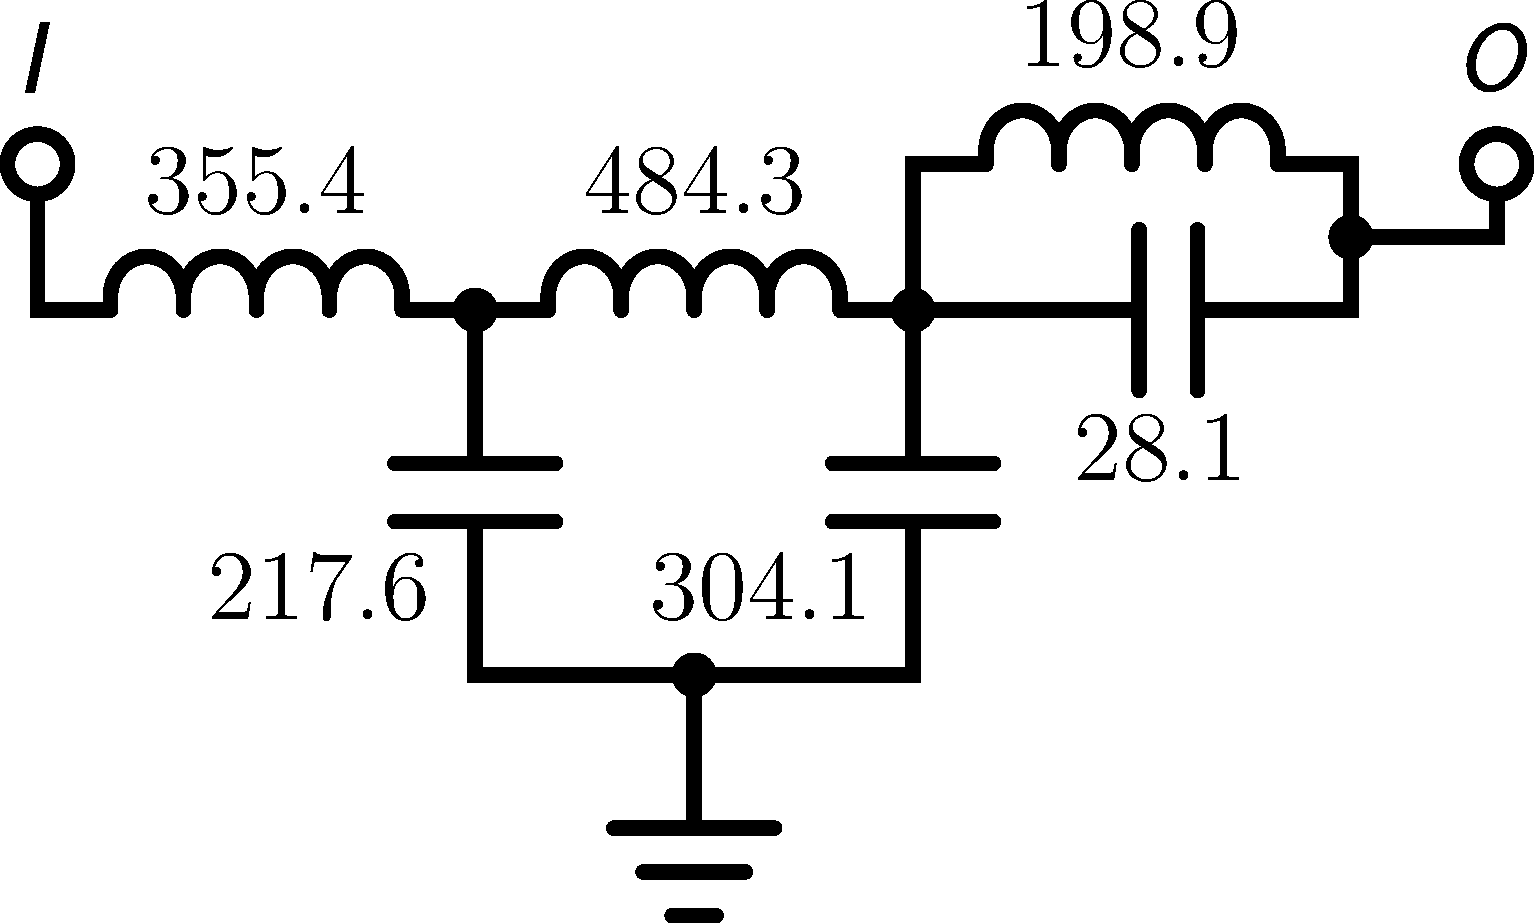
\includegraphics[scale = 0.14]{../ch6/figures/lpf3_circuit2}
\caption{\label{fig:lpf3_circuitb}}
\end{subfigure}%
\begin{subfigure}[t]{0.25\textwidth}
\centering
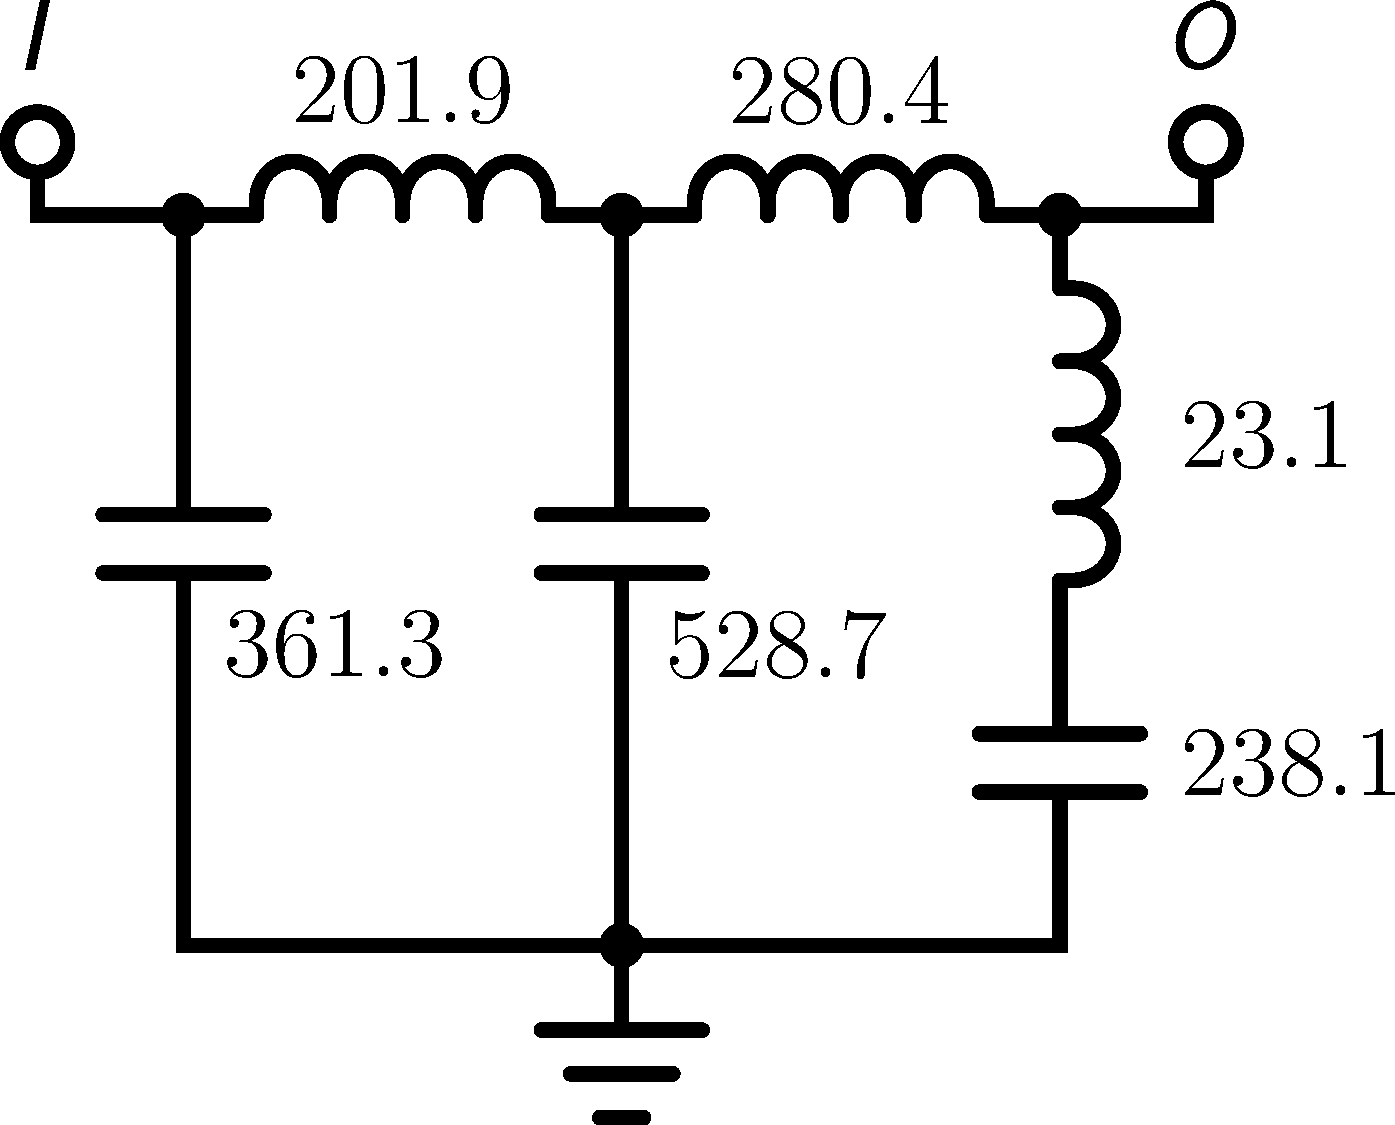
\includegraphics[scale = 0.14]{../ch6/figures/lpf3_circuit3}
\caption{\label{fig:lpf3_circuitc}}
\end{subfigure}%
\begin{subfigure}[t]{0.25\textwidth}
\centering
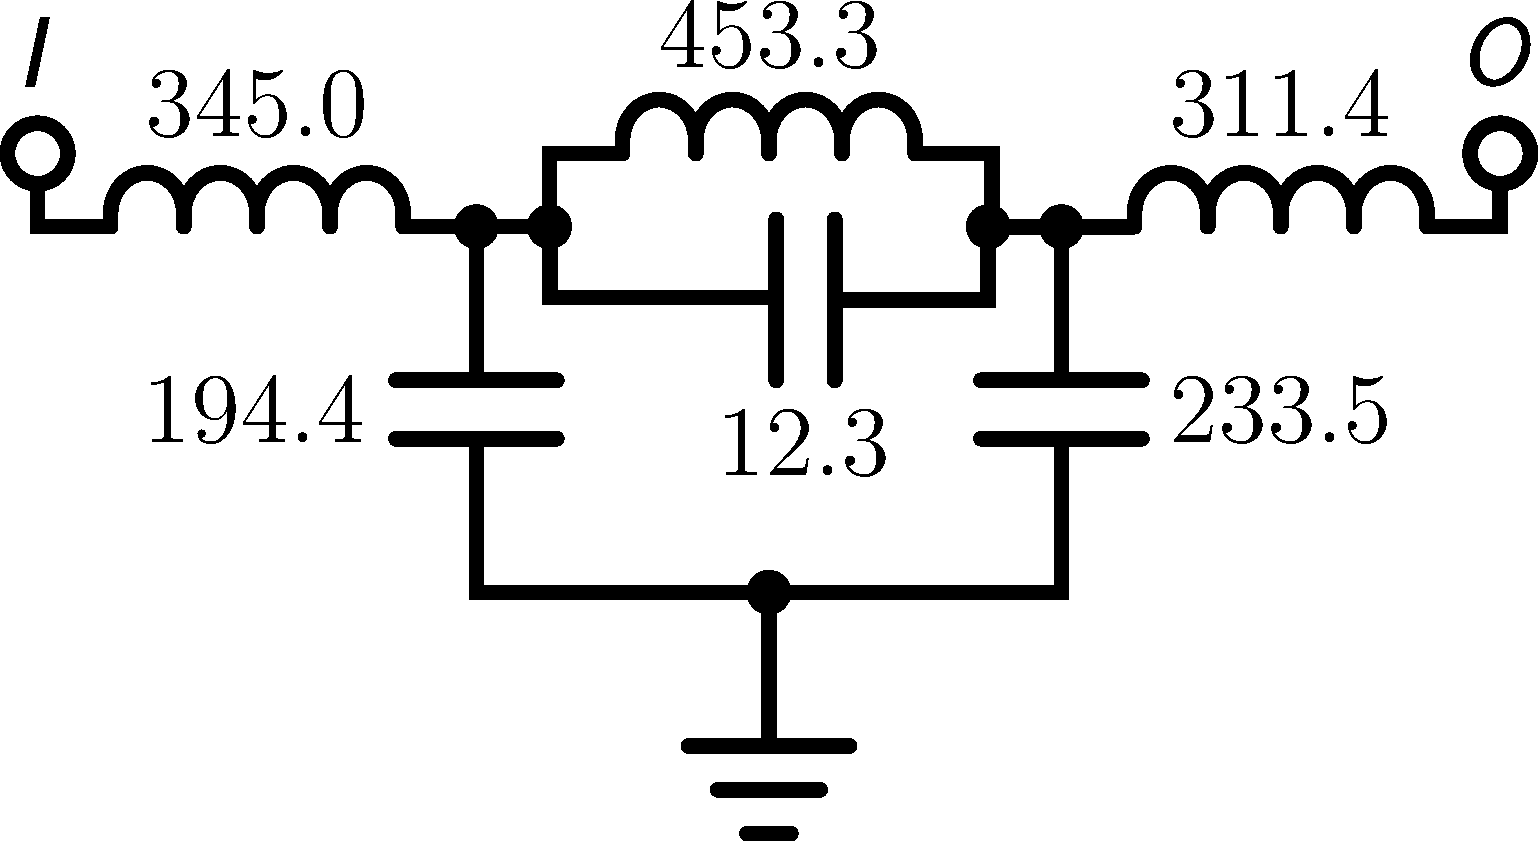
\includegraphics[scale = 0.14]{../ch6/figures/lpf3_circuit4}
\caption{\label{fig:lpf3_circuitd}}
\end{subfigure}%
\vspace{0.06in}
\begin{subfigure}[t]{\textwidth}
\centering
% 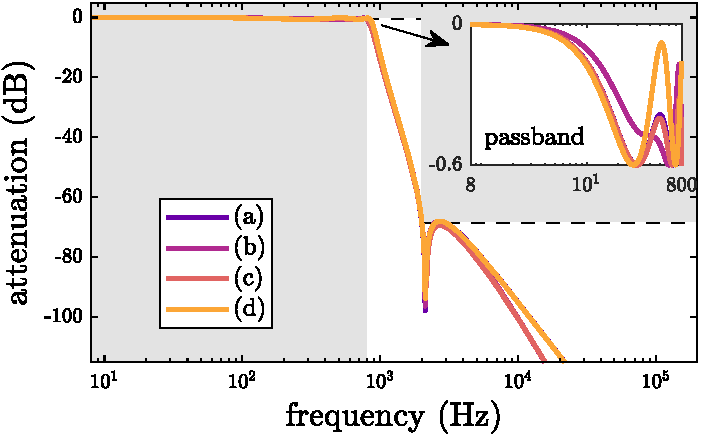
\includegraphics[width=\textwidth]{../ch6/figures/lpf3_magnitude}
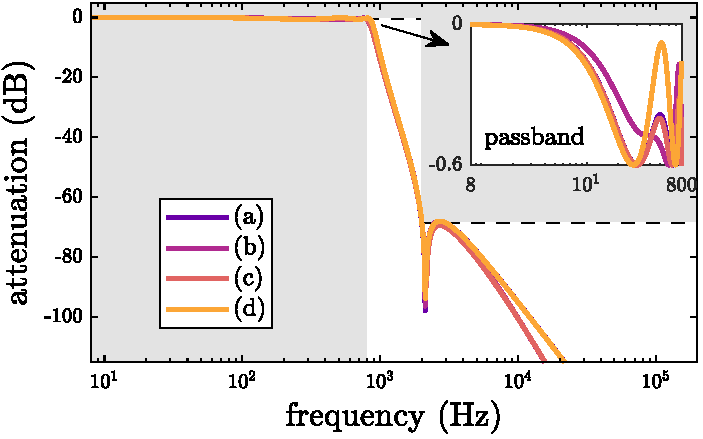
\includegraphics[width=0.5\textwidth]{../ch6/figures/reduced/r_lpf3_magnitude}
\caption{\label{fig:lpf3_magnitude}}
\end{subfigure}%

\caption[Select feasible, minimum complexity circuits and attenuation responses for \nameref{sec:ch6:lpf} task \#3.]{Select feasible, minimum complexity circuits and attenuation responses for \nameref{sec:ch6:lpf} task \#3 (units are mH and nF).\label{fig:lpf3}}

\end{figure}